\chapter{Enolen, enolaten en de aldolreactie}\label{ch:b2:enolates-aldol}

Telkens wanneer een cel glucose afbreekt, knipt een enzym een suikerfosfaat met zes koolstofatomen
in twee stukken van drie koolstofatomen: een \omterm{def:b2:enolates-aldol:aldol}{aldolreactie} die achteruit loopt. Vooruit
verbindt dezelfde reactie twee carbonylverbindingen tot één, en ze is
de meest gebruikte manier van de chemicus om koolstof--koolstofbindingen te maken. Ze berust op een
eigenschap die de vorige hoofdstukken slechts aanstipten: de waterstofatomen naast een
carbonylgroep zijn zuur, en wie er één weghaalt, maakt van het koolstofatoom naast de
carbonylgroep een nucleofiel.

\begin{recall}
Het deel van jaar~1: $\mathrm pK_a$ en de predominante reactie, carbanionen, kinetische en
thermodynamische controle, \omterm{def:b2:amines:nucleophilic-addition}{nucleofiele addities} aan carbonylgroepen, E1- en E2-eliminaties, de hydratatie van
alkynen (een \omterm{def:b2:enolates-aldol:tautomerism}{enol} dat omlegt). \Cref{ch:b2:frontier-orbitals}: ambidente nucleofielen.
\Cref{ch:b2:acyl-substitution}: esters en acylsubstitutie.
\end{recall}

\section{Keto-enoltautomerie}

\begin{definition}[Tautomerie]\label{def:b2:enolates-aldol:tautomerism}
\emph{Tautomeren}\index{tautomeren} zijn isomeren die in elkaar overgaan door verplaatsing van een waterstofatoom en een dubbele
binding. Bij \emph{keto-enoltautomerie}\index{keto-enoltautomerie} staat een carbonylverbinding met een
waterstofatoom op het koolstofatoom naast de carbonylgroep (de ketovorm) in evenwicht met haar
\emph{enol}\index{enol}, een alcohol die door een dubbele binding \ce{C=C} gedragen wordt.
\end{definition}

\begin{omfigure}
\setchemfig{atom sep=2em}
\schemestart
\chemfig{H_3C-C(=[2]O)-CH_3}
\arrow{<=>[\ce{H+} of \ce{HO-}][katalyse]}[,2.2]
\chemfig{H_3C-C(-[2]OH)=CH_2}
\schemestop
\par\vspace{6pt}

{\small Propanon en zijn \omterm{def:b2:enolates-aldol:tautomerism}{enol}, prop-1-een-2-ol. Zuur (protonering van het carbonylzuurstofatoom, daarna verlies
van een $\alpha$-waterstofatoom) of base (wegname van een $\alpha$-waterstofatoom, daarna protonering van het zuurstofatoom)
katalyseert de omzetting; het evenwicht ligt ver aan de kant van de ketovorm.}
\end{omfigure}

\begin{proposition}[Enolgehalte]\label{prop:b2:enolates-aldol:enol-content}
Eenvoudige aldehyden en ketonen bevatten slechts sporen \omterm{def:b2:enolates-aldol:tautomerism}{enol}; 1,3-dicarbonylverbindingen zoals
pentaan-2,4-dion bevatten er een groot deel van.
\end{proposition}

\begin{proof}[Redenering]
Een binding \ce{C=O} is sterker dan een binding \ce{C=C}, en dat verschil is groter dan het verschil waarmee een binding \ce{O-H} zwakker is dan een binding \ce{C-H}:
de ketovorm wordt begunstigd. In een 1,3-dicarbonylverbinding is de dubbele binding van het \omterm{def:b2:enolates-aldol:tautomerism}{enol} geconjugeerd
met de tweede carbonylgroep, en de \ce{OH} van het \omterm{def:b2:enolates-aldol:tautomerism}{enol} vormt een interne waterstofbrug met het zuurstofatoom daarvan,
in een zesring: beide stabiliseren het \omterm{def:b2:enolates-aldol:tautomerism}{enol} genoeg om er een hoofdvorm van te maken.
\end{proof}

Omdat het \omterm{def:b2:enolates-aldol:tautomerism}{enol} vlak is aan zijn \ce{C=C}, gaat een stereocentrum op het $\alpha$-koolstofatoom verloren telkens wanneer
het \omterm{def:b2:enolates-aldol:tautomerism}{enol} zich vormt: een optisch actief keton met een stereocentrum naast zijn carbonylgroep racemiseert in zuur
of in base.

\section{Enolaten}

\begin{definition}[Enolaten]\label{def:b2:enolates-aldol:enolate}
Het \emph{$\alpha$-koolstofatoom}\index{alfa-koolstofatoom@$\alpha$-koolstofatoom} van een carbonylverbinding is het koolstofatoom
dat aan het carbonylkoolstofatoom gebonden is; zijn waterstofatomen zijn \emph{$\alpha$-waterstofatomen}\index{alfa-waterstofatoom@$\alpha$-waterstofatoom}.
Wie er één weghaalt, krijgt een \emph{enolaation}\index{enolaation}, waarvan de
negatieve lading verdeeld is over het $\alpha$-koolstofatoom en het zuurstofatoom.
\end{definition}

\begin{proposition}[Zuurgraad van $\alpha$-waterstofatomen]\label{prop:b2:enolates-aldol:alpha-acidity}
$\alpha$-Waterstofatomen zijn veel zuurder dan gewone bindingen \ce{C-H}, omdat het \omterm{def:b2:enolates-aldol:enolate}{enolaat} gestabiliseerd wordt
door resonantie; een waterstofatoom tussen twee carbonylgroepen is zuur genoeg om door een alkoxide of
zelfs door hydroxide weggehaald te worden.
\end{proposition}

\begin{proof}[Redenering]
In het \omterm{def:b2:enolates-aldol:enolate}{enolaat} zit de negatieve lading gedeeltelijk op het elektronegatieve zuurstofatoom; een tweede carbonylgroep aan
de andere kant delokaliseert haar over twee zuurstofatomen. Gemeten in water heeft pentaan-2,4-dion $\mathrm pK_a =
9.0$ en ethyl-3-oxobutanoaat 10.7, vergelijkbaar met nitromethaan (10.2), waarvan het anion op dezelfde manier
door de nitrogroep gestabiliseerd wordt; een eenvoudig keton, met maar één carbonylgroep, is veel zwakker --- te zwak
om zijn zuurgraad rechtstreeks in water te meten.
% ledger: pka:acac, pka:acetoacetate, pka:nitromethane
\end{proof}

\begin{omfigure}
\setchemfig{atom sep=2em}
\schemestart
\chemfig{H_3C-C(=[2]O)-\chemabove{C}{\scriptstyle -}H_2}
\arrow{<->}
\chemfig{H_3C-C(-[2]\chemabove{O}{\scriptstyle -})=CH_2}
\schemestop
\par\vspace{6pt}

{\small De twee resonantiestructuren van het \omterm{def:b2:enolates-aldol:enolate}{enolaat} van propanon. De negatieve lading wordt gedeeld door
het $\alpha$-koolstofatoom en het zuurstofatoom: het \omterm{def:b2:enolates-aldol:enolate}{enolaat} is een \omterm{def:b2:frontier-orbitals:ambident}{ambident nucleofiel}, dat met de meeste koolstofelektrofielen
op koolstof reageert.}
\end{omfigure}

\begin{definition}[Kinetische en thermodynamische enolaten]\label{def:b2:enolates-aldol:kinetic-enolate}
Bij een keton met twee verschillende $\alpha$-koolstofatomen is het \emph{kinetische enolaat}\index{kinetisch enolaat}
het \omterm{def:b2:enolates-aldol:enolate}{enolaat} dat sneller gevormd wordt, door wegname van een waterstofatoom aan de minst gehinderde, minst gesubstitueerde kant; het
\emph{thermodynamische enolaat}\index{thermodynamisch enolaat} is het stabielere, met de meest
gesubstitueerde dubbele binding.
\end{definition}

\begin{proposition}[Het enolaat kiezen]\label{prop:b2:enolates-aldol:enolate-control}
Een sterke, omvangrijke base die volledig ingezet wordt bij lage temperatuur (lithiumdiisopropylamide, LDA, bij
\qty{-78}{\degreeCelsius}) vormt het \omterm{def:b2:enolates-aldol:kinetic-enolate}{kinetische enolaat} volledig en onomkeerbaar; een zwakkere base bij
kamertemperatuur (een alkoxide in zijn alcohol) laat de \omterm{def:b2:enolates-aldol:enolate}{enolaten} in elkaar overgaan en geeft vooral het
thermodynamische.
\end{proposition}

\begin{proof}[Redenering]
LDA ($\mathrm pK_a$ van diisopropylamine rond 36, ver boven die van het keton) deprotoneert volledig en
snel; bij lage temperatuur wordt het \omterm{def:b2:enolates-aldol:enolate}{enolaat} niet opnieuw geprotoneerd, en de snelste deprotonering, aan de
bereikbare \ce{CH2} of \ce{CH3}, beslist: kinetische controle. Een alkoxide haalt het proton slechts gedeeltelijk weg,
de \omterm{def:b2:enolates-aldol:enolate}{enolaten} en het keton wisselen voortdurend protonen uit, en het evenwichtsmengsel begunstigt het
meest gesubstitueerde, stabielste \omterm{def:b2:enolates-aldol:enolate}{enolaat}: thermodynamische controle (zoals in het deel van jaar~1).
% ledger: ghs:LDA
\end{proof}

\section{Enolaten alkyleren}

\omterm{def:b2:enolates-aldol:enolate}{Enolaten} vallen primaire halogeenalkanen aan door bimoleculaire substitutie, en vormen zo een nieuwe binding \ce{C-C} op
het $\alpha$-koolstofatoom. Met de zeer zure $\alpha$-waterstofatomen van een 1,3-dicarbonylverbinding volstaat een alkoxide,
en de extra carbonylgroep kan achteraf verwijderd worden.

\begin{definition}[Decarboxylering]\label{def:b2:enolates-aldol:decarboxylation}
Een \emph{decarboxylering}\index{decarboxylering} verwijdert een carboxylgroep als \ce{CO2}. Bij de
\emph{malonestersynthese}\index{malonestersynthese} wordt diethylpropaandioaat gedeprotoneerd,
gealkyleerd, gehydrolyseerd tot het gesubstitueerde propaandizuur en door verhitting gedecarboxyleerd, wat een
carbonzuur \ce{RCH2COOH} geeft.
\end{definition}

\begin{proposition}[Gemakkelijke decarboxyleringen]\label{prop:b2:enolates-aldol:decarboxylation}
$\beta$-Ketozuren en propaandizuren verliezen \ce{CO2} bij zacht verwarmen; gewone carbonzuren
niet.
\end{proposition}

\begin{proof}[Redenering]
De carbonylgroep twee bindingen van de carboxylgroep verwijderd neemt het waterstofatoom van \ce{COOH} op in een cyclische
zesledige overgangstoestand terwijl \ce{CO2} vertrekt: er vormt zich rechtstreeks een \omterm{def:b2:enolates-aldol:tautomerism}{enol}, dat daarna tautomeriseert. Zonder
die carbonylgroep heeft het carbanion dat het verlies van \ce{CO2} zou achterlaten geen stabilisatie.
\end{proof}

\begin{definition}[Haloformreactie]\label{def:b2:enolates-aldol:haloform}
De \emph{haloformreactie}\index{haloformreactie} zet een methylketon \ce{RCOCH3}, met een
halogeen en een overmaat hydroxide, om in een carboxylaat \ce{RCOO-} en een haloform \ce{CHX3}.
\end{definition}

Elk ingevoerd halogeenatoom maakt de resterende $\alpha$-waterstofatomen zuurder, zodat de methylgroep
driemaal gehalogeneerd wordt; de groep \ce{CX3-} is dan een voldoende goede vertrekkende groep om door hydroxide uitgestoten te worden in een
acylsubstitutie. Met jood is het gele neerslag van jodoform een test op methylketonen.

\section{De aldolreactie}

\begin{definition}[Aldolreacties]\label{def:b2:enolates-aldol:aldol}
Bij een \emph{aldoladditie}\index{aldoladditie} addeert het \omterm{def:b2:enolates-aldol:enolate}{enolaat} (of \omterm{def:b2:enolates-aldol:tautomerism}{enol}) van een carbonylverbinding
aan de carbonylgroep van een andere, wat een $\beta$-hydroxycarbonylverbinding geeft, een
\emph{aldol}\index{aldol}. Bij een \emph{aldolcondensatie}\index{aldolcondensatie} verliest het aldol
water, wat een $\alpha,\beta$-onverzadigde carbonylverbinding geeft (een enon of enal).
\end{definition}

\begin{omfigure}
\setchemfig{atom sep=1.9em}
\schemestart
\chemfig{H_3C-CH=O} \+ \chemfig{^{-}CH_2-CH=O}
\arrow{->[additie]}
\chemfig{H_3C-CH(-[2]O^{-})-CH_2-CH=O}
\schemestop

\medskip
\schemestart
\arrow{->[\ce{H2O}][$-$ \ce{HO-}]}
\chemfig{H_3C-CH(-[2]OH)-CH_2-CH=O}
\arrow{->[verhitten, base][$-$ \ce{H2O}]}
\chemfig{H_3C-CH=CH-CH=O}
\schemestop
\par\vspace{6pt}

{\small De \omterm{def:b2:enolates-aldol:aldol}{aldolreactie} van ethanal. Het \omterm{def:b2:enolates-aldol:enolate}{enolaat} addeert aan een tweede molecuul ethanal; protonering
geeft het \omterm{def:b2:enolates-aldol:aldol}{aldol}, 3-hydroxybutanal. Bij verhitten met base wordt een $\alpha$-waterstofatoom weggehaald en vertrekt hydroxide
van het $\beta$-koolstofatoom: but-2-enal, geconjugeerd.}
\end{omfigure}

\begin{proposition}[De aldolreactie voortdrijven]\label{prop:b2:enolates-aldol:aldol-equilibrium}
De \omterm{def:b2:enolates-aldol:aldol}{aldoladditie} is omkeerbaar; de dehydratatie, die een geconjugeerd systeem vormt, trekt de
reactie naar het condensatieproduct.
\end{proposition}

\begin{proof}[Redenering]
Twee moleculen geven er één, dus de \omterm{def:b2:reaction-free-energy:reaction-entropy}{reactie-entropie} is negatief, en de nieuwe binding \ce{C-C} weegt nauwelijks
op tegen de verloren $\pi$-binding van \ce{C=O}: voor veel ketonen is $K$ klein. Het \omterm{def:b2:enolates-aldol:aldol}{aldol} wegnemen door dehydratatie
houdt $Q < K$ voor de additie; het gevormde geconjugeerde enon is gestabiliseerd en, bij hoge temperatuur,
begunstigt de entropiewinst van het vrijkomende water het nog meer. De omgekeerde reactie, de \omterm{def:b2:enolates-aldol:aldol}{retro-aldolreactie}, is de
stap waarmee de cel een suiker met zes koolstofatomen splitst.
\end{proof}

\begin{method}[Een gekruiste aldolreactie sturen]\label{met:b2:enolates-aldol:crossed-aldol}
\begin{enumerate}
  \item Gebruik een partner zonder $\alpha$-waterstofatomen (benzaldehyde, methanal): die kan alleen het
        elektrofiel zijn.
  \item Of vorm eerst volledig het \omterm{def:b2:enolates-aldol:enolate}{enolaat} van een partner (LDA, \qty{-78}{\degreeCelsius}), en voeg daarna
        de andere toe.
  \item Of gebruik een 1,3-dicarbonylpartner, veel zuurder dan de andere.
  \item Verkies een aldehyde als elektrofiel: het is reactiever dan een keton.
\end{enumerate}
\end{method}

\begin{method}[Een aldolproduct herkennen]\label{met:b2:enolates-aldol:aldol-recognition}
\begin{enumerate}
  \item Zoek een \ce{C=O} met een \ce{OH} op het koolstofatoom twee atomen verder ($\beta$), of een \ce{C=C}
        die geconjugeerd is met een \ce{C=O}.
  \item Knip de binding tussen het $\alpha$- en het $\beta$-koolstofatoom door: het $\beta$-koolstofatoom was een carbonylkoolstofatoom (het
        elektrofiel), het $\alpha$-koolstofatoom het koolstofatoom van het \omterm{def:b2:enolates-aldol:enolate}{enolaat}.
  \item Controleer dat beide partners bestaan en dat het \omterm{def:b2:enolates-aldol:enolate}{enolaat} selectief gevormd kan worden.
\end{enumerate}
\end{method}

\section{De claisencondensatie}

\begin{definition}[Claisencondensatie]\label{def:b2:enolates-aldol:claisen}
Bij een \emph{claisencondensatie}\index{claisencondensatie} valt het \omterm{def:b2:enolates-aldol:enolate}{enolaat} van een ester de
carbonylgroep van een ander estermolecuul aan in een acylsubstitutie, wat een \emph{$\beta$-ketoester}\index{beta-ketoester@$\beta$-ketoester}
geeft en een alkoxide vrijmaakt. De intramoleculaire versie ervan, de cyclisatie van
Dieckmann, geeft een cyclische $\beta$-ketoester.
\end{definition}

\begin{proposition}[Wat de claisencondensatie voortdrijft]\label{prop:b2:enolates-aldol:claisen-drive}
De \omterm{def:b2:enolates-aldol:claisen}{claisencondensatie} van ethylethanoaat vraagt een volledig equivalent natriumethoxide: haar evenwicht
is ongunstig, en ze wordt voortgedreven door de deprotonering van de gevormde $\beta$-ketoester.
\end{proposition}

\begin{proof}
De eigenlijke condensatie, \ce{2CH3COOEt <=> CH3COCH2COOEt + EtOH}, heeft een kleine evenwichtsconstante
$K_1$. De $\beta$-ketoester ($\mathrm pK_a = 10.7$) wordt daarna gedeprotoneerd door ethoxide (ethanol, 15.9):
$K_2 = 10^{15.9 - 10.7} = 10^{5.2}$. De totale reactie, condensatie plus deprotonering, heeft
$K_1K_2$, groot genoeg zelfs bij een kleine $K_1$; de base wordt verbruikt en een zure opwerking geeft de neutrale
$\beta$-ketoester. Een ester met maar één $\alpha$-waterstofatoom, waarvan het product niet gedeprotoneerd kan worden, geeft
weinig product.
% ledger: pka:acetoacetate, pka:ethanol
\end{proof}

\begin{history}[Het aldol, 1872]
\begin{minipage}[t]{0.18\linewidth}
\vspace{0pt}
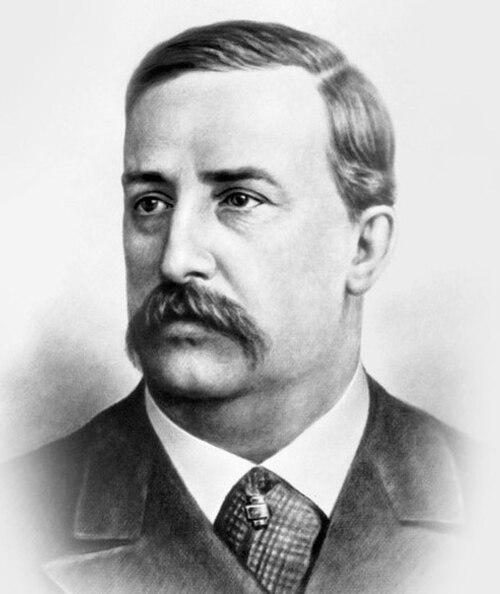
\includegraphics[width=\linewidth]{images/book3/borodin.jpg}
\end{minipage}\hspace{0.02\linewidth}%
\begin{minipage}[t]{0.18\linewidth}
\vspace{0pt}
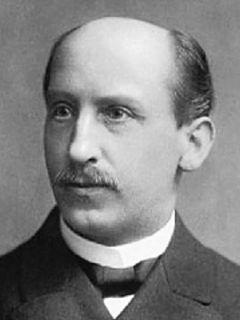
\includegraphics[width=\linewidth]{images/book3/claisen.jpg}
\end{minipage}\hfill
\begin{minipage}[t]{0.58\linewidth}
\vspace{0pt}
De \omterm{def:b2:enolates-aldol:aldol}{aldolreactie} werd in 1872 beschreven door Charles-Adolphe Wurtz en, onafhankelijk daarvan, door Alexander
Borodin, een chemicus in Sint-Petersburg die vandaag beter bekend is als de componist van \textit{Prins Igor}.
Ludwig Claisen breidde de condensaties van carbonylverbindingen in 1887 uit tot esters. (Portretten: Borodin,
onbekende auteur, publiek domein; Claisen, door Veronica.villagrasa, CC BY-SA 4.0; Wikimedia Commons.)
\end{minipage}
\end{history}

\begin{safety}{\ghs[5mm]{GHS02}\,\ghs[5mm]{GHS05}\,\ghs[5mm]{GHS07}}
Natriumethoxide en lithiumdiisopropylamide zijn corrosief en reageren met water; LDA-oplossingen zijn
ontvlambaar en worden onder inert gas gehanteerd. Benzaldehyde en propanon zijn schadelijk en ontvlambaar.
% ledger: ghs:NaOEt, ghs:LDA, ghs:benzaldehyde, ghs:acetone
\end{safety}

\section{Oefeningen}

\begin{exercise}[$\star$]\label{exo:b2:enolates-aldol:1}
Teken de enoltautomeren van butanon en van cyclohexanon.
\end{exercise}

\begin{exercise}[$\star$]\label{exo:b2:enolates-aldol:2}
Rangschik naar de zuurgraad van hun zuurste \ce{C-H}: propanon, pentaan-2,4-dion, ethyl-3-oxobutanoaat,
ethaan.
\end{exercise}

\begin{exercise}[$\star$]\label{exo:b2:enolates-aldol:3}
Geef het \omterm{def:b2:enolates-aldol:aldol}{aldol} en het condensatieproduct van ethanal met natriumhydroxide.
\end{exercise}

\begin{exercise}[$\star$]\label{exo:b2:enolates-aldol:4}
Schrijf de \omterm{def:b2:enolates-aldol:decarboxylation}{malonestersynthese} van hexaanzuur op: welk halogeenalkaan is nodig?
\end{exercise}

\begin{exercise}[$\star\star$]\label{exo:b2:enolates-aldol:5}
Teken het kinetische en het \omterm{def:b2:enolates-aldol:kinetic-enolate}{thermodynamische enolaat} van 2-methylcyclohexanon en de omstandigheden die
elk ervan geven.
\end{exercise}

\begin{exercise}[$\star\star$]\label{exo:b2:enolates-aldol:6}
Geef het product van de gekruiste \omterm{def:b2:enolates-aldol:aldol}{aldolcondensatie} van benzaldehyde met propanon (één equivalent
van elk) en leg uit waarom benzaldehyde niet met zichzelf condenseert.
\end{exercise}

\begin{exercise}[$\star\star$]\label{exo:b2:enolates-aldol:7}
Hexaan-2,5-dion ondergaat in base een intramoleculaire \omterm{def:b2:enolates-aldol:aldol}{aldolcondensatie}. Welke ring ontstaat? Verklaar de
keuze tussen de mogelijke ringen.
\end{exercise}

\begin{exercise}[$\star\star$]\label{exo:b2:enolates-aldol:8}
Schrijf de \omterm{def:b2:enolates-aldol:claisen}{claisencondensatie} van ethylethanoaat op en het product ervan na zure opwerking.
\end{exercise}

\begin{exercise}[$\star\star$]\label{exo:b2:enolates-aldol:9}
Welke van deze verbindingen geven een positieve jodoformtest: propanon, pentaan-3-on, ethanal, acetofenon?
\end{exercise}

\begin{exercise}[$\star\star\star$]\label{exo:b2:enolates-aldol:10}
Schrijf de cyclisatie van Dieckmann van diethylhexaandioaat op en de ringgrootte van het product.
\end{exercise}

\begin{exercise}[$\star\star\star$]\label{exo:b2:enolates-aldol:11}
(\textit{R})-3-Methylpentaan-2-on verliest zijn optische activiteit in verdund natriumhydroxide, maar
(\textit{R})-4-methylhexaan-2-on niet. Leg uit.
\end{exercise}

\begin{exercise}[$\star\star\star$]\label{exo:b2:enolates-aldol:12}
Stel een route voor naar 1,5-difenylpenta-1,4-dieen-3-on, en daarna naar een dienon met twee verschillende arylgroepen,
en zeg waarom het tweede moeilijker is.
\end{exercise}

\section{Probleem: dibenzalaceton}

\begin{problem}[{Weekendprobleem --- het enolaat van propanon en de rol van benzaldehyde, de twee
aldolcondensaties, het geconjugeerde product, en de stoichiometrie en het rendement van een bereiding}]
\label{pb:b2:enolates-aldol:1}
Bereiding (gegevens voor de oefening): \qty{2.1}{mL} benzaldehyde en \qty{0.75}{mL} propanon worden geroerd
in ethanol met waterig natriumhydroxide; gele kristallen van 1,5-difenylpenta-1,4-dieen-3-on
(dibenzalaceton) scheiden zich af; rendement 75~\%. Dichtheden (\unit{g/cm^3}): benzaldehyde 1.045, propanon 0.7845.
Molaire massa's (\unit{g/mol}): C 12.011, H 1.008, O 15.999.
% ledger: rho:benzaldehyde, rho:acetone, aw:C, aw:H, aw:O, ghs:dibenzalacetone

\medskip
\noindent\textbf{Deel I --- De partners.}
\begin{enumerate}
  \item Welke partner heeft $\alpha$-waterstofatomen? Hoeveel?
  \item Teken het \omterm{def:b2:enolates-aldol:enolate}{enolaat} van propanon.
  \item Waarom kan benzaldehyde geen \omterm{def:b2:enolates-aldol:enolate}{enolaat} vormen?
  \item Waarom reageert propanon met benzaldehyde en niet met zichzelf?
  \item Waarom is een aldehyde een beter elektrofiel dan een keton?
  \item Waarom volstaat hydroxide hier als base?
\end{enumerate}

\medskip
\noindent\textbf{Deel II --- Het mechanisme.}
\begin{enumerate}[resume]
  \item Schrijf de additie van het \omterm{def:b2:enolates-aldol:enolate}{enolaat} aan benzaldehyde op.
  \item Schrijf de dehydratatie van het gevormde \omterm{def:b2:enolates-aldol:aldol}{aldol} op.
  \item Waarom verloopt de dehydratatie hier gemakkelijk?
  \item Waarom kan de reactie een tweede keer plaatsvinden?
  \item Schrijf de totale vergelijking op.
  \item Wat drijft de reactie in deze bereiding tot volledigheid?
\end{enumerate}

\medskip
\noindent\textbf{Deel III --- Het product.}
\begin{enumerate}[resume]
  \item Hoeveel dubbele bindingen \ce{C=C} heeft dibenzalaceton, en met welke configuratie (vooral)?
  \item Waarom wordt het (\textit{E},\textit{E})-isomeer begunstigd?
  \item Tel de geconjugeerde $\pi$-bindingen.
  \item Waarom is de verbinding geel, terwijl haar partners kleurloos zijn?
  \item Is dibenzalaceton chiraal?
\end{enumerate}

\medskip
\noindent\textbf{Deel IV --- Stoichiometrie en rendement.}
\begin{enumerate}[resume]
  \item Bereken de molaire massa's van benzaldehyde, propanon en dibenzalaceton.
  \item Bereken de hoeveelheden van de twee reagentia.
  \item Welk reagens is beperkend?
  \item Bereken de theoretische massa product.
  \item Waarom is een lichte overmaat benzaldehyde te verkiezen boven een overmaat propanon?
  \item Wat zou een overmaat propanon geven?
  \item Geef de massa dibenzalaceton die verkregen wordt bij een rendement van 75~\%.
\end{enumerate}
\end{problem}
